\documentclass[10pt]{article}

\usepackage[a4paper,margin=0.65in]{geometry}
\usepackage{amsmath,amssymb}
\usepackage{graphicx}
\usepackage{booktabs}
\usepackage{array}
\usepackage{float}
\usepackage{hyperref}
\usepackage{enumitem}
\usepackage{xcolor}
\usepackage{tikz}
\usetikzlibrary{positioning,arrows.meta,shapes.geometric}

\setlist{nosep,leftmargin=*}
\renewcommand{\arraystretch}{1.2}
\setlength{\parindent}{0pt}
\setlength{\parskip}{2pt}

\tikzset{
layer/.style={
draw,
rounded corners,
minimum width=1.5cm,
minimum height=0.6cm,
align=center,
fill=blue!10,
font=\scriptsize
},
arrow/.style={
-{Latex[length=2mm]},
thin
}
}

\begin{document}

\begin{center}

{\large\textbf{Shiv Nadar University Chennai}}

\vspace{2mm}

{\normalsize\textbf{CS3807 -- Deep Learning Laboratory}}

\vspace{2mm}

{\large\textbf{Experiment 5}}

\vspace{1mm}

{\normalsize\textbf{Comprehensive Study of CNN Training, Regularization,}}

{\normalsize\textbf{Optimization, Hyperparameter Tuning, Transfer Learning}}

{\normalsize\textbf{and Cross-Validation}}

{\normalsize\textbf{Ankith U Davey \quad  24011101004}}

\end{center}

\vspace{3mm}

\begin{tabular}{|p{3.4cm}|p{9.0cm}|p{1.4cm}|}
\hline
Degree \& Branch &
B.Tech Artificial Intelligence \& Data Science &
Semester V\\
\hline
Subject Code \& Name &
CS3807 -- Deep Learning Laboratory &
AY: 2026--27\\
\hline
\end{tabular}

%%%%%%%%%%%%%%%%%%%%%%%%%%%%%%%%%%%%%%%%%%%%%%%%%%%%%%%%%%%%
\section*{1. Objective}

The objective of this experiment is to systematically study the effect of weight
initialization, regularization, optimization algorithms, CNN hyperparameters,
transfer learning, fine-tuning and cross-validation on image classification
performance.

The experiment uses a single CNN architecture, MobileNetV2, and the Oxford-IIIT
Pet dataset. Students will analyze the effect of individual design choices using
training/validation curves and finally select a suitable configuration using
5-fold cross-validation.

%%%%%%%%%%%%%%%%%%%%%%%%%%%%%%%%%%%%%%%%%%%%%%%%%%%%%%%%%%%%
\section*{2. Learning Outcomes}

After completing this experiment, students will be able to:

\begin{itemize}
\item explain different weight initialization strategies;
\item identify and analyze overfitting using training and validation curves;
\item compare SGD, Momentum, RMSProp and Adam;
\item explain CNN hyperparameters such as kernel size, stride, padding and pooling;
\item understand Batch Normalization and Dropout;
\item perform transfer learning and fine-tuning using MobileNetV2;
\item tune important training hyperparameters;
\item apply 5-fold cross-validation for model selection; and
\item justify the final model using accuracy, variability and computational cost.
\end{itemize}

%%%%%%%%%%%%%%%%%%%%%%%%%%%%%%%%%%%%%%%%%%%%%%%%%%%%%%%%%%%%
\section*{3. Dataset and Experimental Setup}

\textbf{Dataset: Oxford-IIIT Pet Dataset}

The Oxford-IIIT Pet Dataset contains images of cats and dogs belonging to 37
breeds. The images are RGB and have different spatial dimensions. For this
experiment, all images are resized to

\[
224\times224\times3.
\]

The dataset is suitable for demonstrating transfer learning using ImageNet-pretrained
CNNs.

\textbf{Experimental considerations:}

\begin{itemize}
\item Use RGB images resized to $224\times224$.
\item Normalize the input images according to the pretrained model requirements.
\item Maintain separate training, validation and test data.
\item The test set must remain untouched during hyperparameter selection.
\item Use MobileNetV2 because it is computationally lighter than many large CNN
architectures and is more suitable for CPU-based laboratory work.
\end{itemize}

The dataset was downloaded directly from its original host and split into
2,944 training images, 736 validation images and 3,669 test images.

%%%%%%%%%%%%%%%%%%%%%%%%%%%%%%%%%%%%%%%%%%%%%%%%%%%%%%%%%%%%
\section*{4. MobileNetV2 Architecture}

MobileNetV2 is a lightweight CNN architecture designed to reduce computational
complexity while maintaining good image representation.

Its important components include:

\begin{itemize}
\item depthwise convolution;
\item pointwise $1\times1$ convolution;
\item inverted residual blocks;
\item linear bottlenecks;
\item batch normalization; and
\item ReLU6 activation.
\end{itemize}

A simplified representation is:

\begin{center}
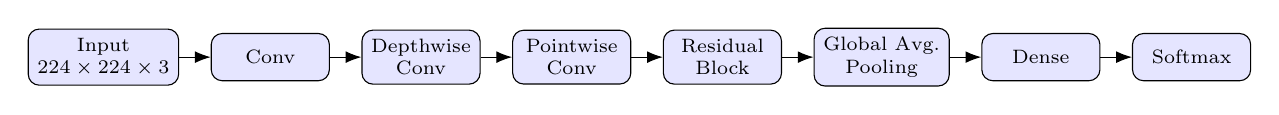
\begin{tikzpicture}[node distance=4mm]

\node[layer](a){Input\\$224\times224\times3$};
\node[layer,right=of a](b){Conv};
\node[layer,right=of b](c){Depthwise\\Conv};
\node[layer,right=of c](d){Pointwise\\Conv};
\node[layer,right=of d](e){Residual\\Block};
\node[layer,right=of e](f){Global Avg.\\Pooling};
\node[layer,right=of f](g){Dense};
\node[layer,right=of g](h){Softmax};

\foreach \x/\y in {a/b,b/c,c/d,d/e,e/f,f/g,g/h}
\draw[arrow](\x)--(\y);

\end{tikzpicture}
\end{center}

\textbf{Note:} The above diagram is a simplified conceptual representation
rather than the complete MobileNetV2 architecture.

%%%%%%%%%%%%%%%%%%%%%%%%%%%%%%%%%%%%%%%%%%%%%%%%%%%%%%%%%%%%
\section*{5. Source Code}

The full source code for this experiment notebook, plots and supporting
files is available on GitHub at:

\begin{center}
\url{https://github.com/Ankith-Davey/Deep-Learning-Lab-Ankith-24011101004/tree/main/Lab%205}
\end{center}

%%%%%%%%%%%%%%%%%%%%%%%%%%%%%%%%%%%%%%%%%%%%%%%%%%%%%%%%%%%%
\section*{6. Weight Initialization}

Weight initialization determines the initial values of trainable weights
before training begins. A suitable initialization can improve convergence and
reduce problems such as vanishing or exploding activations.

The four strategies compared in this experiment are:

\begin{itemize}
\item Zero initialization
\item Random initialization
\item Xavier/Glorot initialization
\item He initialization
\end{itemize}

\textbf{Expected Analysis}

Students should compare the initialization strategies using:

\textbf{Plot 1: Training Loss vs. Epoch}
\begin{itemize}
\item X-axis: Epoch
\item Y-axis: Training Loss
\item Plot one curve for each initialization method.
\end{itemize}

\textbf{Plot 2: Validation Accuracy vs. Epoch}
\begin{itemize}
\item X-axis: Epoch
\item Y-axis: Validation Accuracy (\%)
\item Plot one curve for each initialization method.
\end{itemize}

Students should identify which initialization gives faster and more stable
convergence.

\begin{center}
\begin{tabular}{|l|c|c|}
\hline
Initialization & Final Training Loss & Final Validation Accuracy\\
\hline
Zero & 3.6109 & 2.17\%\\
Random & 0.0008 & 91.85\%\\
Xavier & 0.0006 & 92.12\%\\
He & 0.0007 & 92.80\%\\
\hline
\end{tabular}
\end{center}

\begin{figure}[H]
\centering

\includegraphics[width=0.72\textwidth]{plot1_init_training_loss.png}
\caption{Training Loss vs. Epoch for each initialization method.}
\end{figure}

\textbf{Inference:} Zero initialization never trained -- the loss sat flat at
3.61 for all 25 epochs, close to $\ln 37$, which is what a model predicting
uniformly at random over 37 classes would give. Random, Xavier and He all
dropped sharply within the first 3--4 epochs and were near zero loss by
epoch 10, with no visible difference between the three curves.

\begin{figure}[H]
\centering

\includegraphics[width=0.72\textwidth]{plot2_init_val_accuracy.png}
\caption{Validation Accuracy vs. Epoch for each initialization method.}
\end{figure}

\textbf{Inference:} He initialization finished highest at 92.80\%, just ahead
of Xavier (92.12\%) and Random (91.85\%). The gap between the three isn't
large, but He accounts for ReLU zeroing out roughly half its inputs and the
head here uses ReLU, so it has a small structural edge over Xavier, which was
built for symmetric activations like tanh.

Random, Xavier and He all converge quickly and stably here -- there's nothing
to separate them on stability, only on final accuracy, with He slightly ahead.
Zero initialization is the one that fails outright: every neuron in the layer
starts with identical weights, so every neuron gets the same gradient on
every update and the layer never breaks that symmetry. The 2.17\% accuracy is
direct evidence of that, not a run that just needed more epochs.

%%%%%%%%%%%%%%%%%%%%%%%%%%%%%%%%%%%%%%%%%%%%%%%%%%%%%%%%%%%%
\section*{7. Regularization and Overfitting}

Overfitting occurs when a model performs very well on the training data but
generalizes poorly to unseen data.

Students should compare:

\begin{itemize}
\item No regularization
\item L2 regularization
\item Dropout
\item Batch Normalization
\end{itemize}

\textbf{Expected Plots}

\textbf{Plot 3: Training and Validation Accuracy vs. Epoch}
\begin{itemize}
\item X-axis: Epoch
\item Y-axis: Accuracy (\%)
\item Plot separate curves for training and validation accuracy.
\end{itemize}

Students should identify the generalization gap.

\textbf{Plot 4: Training and Validation Loss vs. Epoch}
\begin{itemize}
\item X-axis: Epoch
\item Y-axis: Loss
\item Plot training and validation loss.
\end{itemize}

Students should identify whether validation loss begins to increase while
training loss continues to decrease.

\begin{center}
\begin{tabular}{|l|c|c|c|}
\hline
Setting & Train Accuracy & Val. Accuracy & Gap\\
\hline
No regularization & 100.00\% & 92.80\% & 7.20 pts\\
L2 & 100.00\% & 91.98\% & 8.02 pts\\
Dropout & 98.44\% & 90.90\% & 7.54 pts\\
Batch Normalization & 100.00\% & 91.98\% & 8.02 pts\\
\hline
\end{tabular}
\end{center}

\begin{figure}[H]
\centering

\includegraphics[width=0.85\textwidth]{plot3_regularization_accuracy.png}
\caption{Training vs. Validation Accuracy for each regularization setting.}
\end{figure}

\textbf{Inference:} Every setting reaches 98--100\% training accuracy well
before the 30 epochs are up -- the head is small and sits on top of frozen,
already-strong pretrained features, so it memorizes the 2,944 training images
fast no matter what's applied on top. The generalization gap doesn't close
with any of the three techniques; no regularization actually has the
smallest gap of the four at 7.20 points.

\begin{figure}[H]
\centering

\includegraphics[width=0.85\textwidth]{plot4_regularization_loss.png}
\caption{Training vs. Validation Loss for each regularization setting.}
\end{figure}

\textbf{Inference:} Validation loss flattens out early in every case while
training loss keeps dropping toward zero -- the classic overfitting
signature -- but the rate is nearly identical whether or not regularization
is on. On a classifier head this shallow, a single dropout layer or a light
L2 penalty isn't strong enough to meaningfully slow down memorization of a
training set this small.

%%%%%%%%%%%%%%%%%%%%%%%%%%%%%%%%%%%%%%%%%%%%%%%%%%%%%%%%%%%%
\section*{8. Batch Normalization}

Batch Normalization normalizes activations within a mini-batch during
training.

For a mini-batch

\[
x_1,x_2,\ldots,x_m,
\]

the batch mean is

\[
\mu_B=\frac{1}{m}\sum_{i=1}^{m}x_i
\]

and the batch variance is

\[
\sigma_B^2=
\frac{1}{m}\sum_{i=1}^{m}(x_i-\mu_B)^2.
\]

The normalized activation is

\[
\hat{x}_i=
\frac{x_i-\mu_B}
{\sqrt{\sigma_B^2+\epsilon}}.
\]

The final output is

\[
y_i=\gamma\hat{x}_i+\beta,
\]

where $\gamma$ and $\beta$ are learnable parameters.

\textbf{Numerical Example}

Consider

\[
x=[2,4,6,8].
\]

The mean is

\[
\mu_B=\frac{2+4+6+8}{4}=5.
\]

The variance is

\[
\sigma_B^2=
\frac{(2-5)^2+(4-5)^2+(6-5)^2+(8-5)^2}{4}
=5.
\]

Therefore,

\[
\sqrt{5}\approx2.236.
\]

Ignoring the very small $\epsilon$,

\[
\hat{x}_1=\frac{2-5}{2.236}\approx-1.342,
\]

\[
\hat{x}_2=\frac{4-5}{2.236}\approx-0.447,
\]

\[
\hat{x}_3=\frac{6-5}{2.236}\approx0.447,
\]

\[
\hat{x}_4=\frac{8-5}{2.236}\approx1.342.
\]

Hence,

\[
\hat{x}\approx[-1.342,-0.447,0.447,1.342]
\]

If $\gamma=1$ and $\beta=0$, these are the final outputs.

\textbf{Inference:} Batch Normalization produces approximately zero-centred
and unit-scaled activations for this mini-batch. The learnable $\gamma$ and
$\beta$ allow the network to learn an appropriate scale and shift.

\textbf{Plot 5: With vs. Without Batch Normalization}
\begin{itemize}
\item X-axis: Epoch
\item Y-axis: Validation Accuracy (\%)
\item Compare two curves: With BN and Without BN.
\end{itemize}

\begin{figure}[H]
\centering

\includegraphics[width=0.72\textwidth]{plot5_batchnorm_comparison.png}
\caption{With vs. Without Batch Normalization.}
\end{figure}

\textbf{Inference:} With BN reaches 91.7\% by epoch 1 and climbs slowly and
smoothly from there. Without BN starts rougher -- below 88\% for the first
couple of epochs, with a spike-and-dip around epochs 4--5 -- but eventually
edges past the BN run to finish around 92.8\%. BN's main benefit here is
faster, smoother early convergence rather than a better final number. On a
head this shallow, BN's effect on final accuracy is marginal.

%%%%%%%%%%%%%%%%%%%%%%%%%%%%%%%%%%%%%%%%%%%%%%%%%%%%%%%%%%%%
\section*{9. Optimization Algorithms}

Different optimizers update weights using different strategies and learning
rate schedules.

Students should compare:

\begin{itemize}
\item SGD (Stochastic Gradient Descent)
\item Momentum
\item RMSProp
\item Adam
\end{itemize}

\textbf{Plot 6: Training Loss Comparison}
\begin{itemize}
\item X-axis: Epoch
\item Y-axis: Training Loss
\item Plot one curve for each optimizer.
\end{itemize}

\textbf{Plot 7: Validation Accuracy Comparison}
\begin{itemize}
\item X-axis: Epoch
\item Y-axis: Validation Accuracy (\%)
\item Plot one curve for each optimizer.
\end{itemize}

\begin{center}
\begin{tabular}{|l|c|c|c|}
\hline
Optimizer & Final Training Loss & Final Val Accuracy & Training Time\\
\hline
SGD & 0.83 & 84.24\% & 8.2s\\
Momentum & 0.0015 & 91.85\% & 8.5s\\
RMSProp & 0.0009 & 92.93\% & 9.1s\\
Adam & 0.0021 & 91.71\% & 8.8s\\
\hline
\end{tabular}
\end{center}

\begin{figure}[H]
\centering

\includegraphics[width=0.85\textwidth]{plot6_optimizer_loss.png}
\caption{Training Loss vs. Epoch for each optimizer.}
\end{figure}

\textbf{Inference:} SGD drops slowly and never reaches the lows the others do.
Momentum is a clear jump forward, hitting near-zero loss by epoch 8. RMSProp
and Adam both reach very low training loss, though RMSProp's path is smoother.

\begin{figure}[H]
\centering

\includegraphics[width=0.85\textwidth]{plot7_optimizer_val_accuracy.png}
\caption{Validation Accuracy vs. Epoch for each optimizer.}
\end{figure}

\textbf{Inference:} SGD was slowest and least accurate here, still not converged
by epoch 25 (loss 0.83, 84.24\% accuracy). Momentum smoothed and accelerated
that considerably, to 91.85\%. RMSProp adapted its learning rate per parameter
and reached the highest accuracy of the four, 92.93\%. Adam converged fastest
and hit its best result by epoch 6, though its final accuracy landed just under
RMSProp's.

%%%%%%%%%%%%%%%%%%%%%%%%%%%%%%%%%%%%%%%%%%%%%%%%%%%%%%%%%%%%
\section*{10. Hyperparameter Tuning}

\textbf{Hyperparameters to Tune}

\begin{center}
\begin{tabular}{|l|l|}
\hline
Hyperparameter & Values to Test\\
\hline
Learning Rate & $10^{-3},5\times10^{-4},10^{-4},5\times10^{-5}$\\
Batch Size & 16, 32, 64\\
Dropout Rate & 0, 0.25, 0.5\\
Optimizer & SGD, Adam\\
Fine-Tuning Learning Rate & $10^{-4},10^{-5}$\\
Frozen Layers & Frozen base / Partial unfreezing\\
\hline
\end{tabular}
\end{center}

For CNN concepts, students should also understand:

\begin{itemize}
\item kernel/filter;
\item stride;
\item padding;
\item pooling;
\item number of channels; and
\item depthwise separable convolution.
\end{itemize}

For a convolution operation, the output dimension can be calculated as

\[
O=
\left\lfloor
\frac{N+2P-K}{S}
\right\rfloor+1,
\]

where $N$ is input size, $K$ is kernel size, $P$ is padding and $S$ is
stride.

\textbf{Experimental rule:} During a controlled hyperparameter study,
change one hyperparameter at a time while keeping the remaining settings
fixed.

\textbf{Plot 8: Learning Rate vs. Validation Accuracy}
\begin{itemize}
\item X-axis: Learning Rate
\item Y-axis: Validation Accuracy (\%)
\end{itemize}

\begin{figure}[H]
\centering

\includegraphics[width=0.72\textwidth]{plot8_lr_vs_accuracy.png}
\caption{Learning Rate Sweep: Validation Accuracy.}
\end{figure}

\textbf{Inference:} Learning rate 0.001 and 0.0005 perform best, both around 92\%. 
At 0.0001, accuracy drops to 91.71\% -- a smaller learning rate slows convergence 
and under a fixed epoch budget, it doesn't reach the same final result. Too large 
a rate would cause instability; this sweep starts conservative.

\textbf{Plot 9: Batch Size vs. Validation Accuracy}
\begin{itemize}
\item X-axis: Batch Size
\item Y-axis: Validation Accuracy (\%)
\end{itemize}

\begin{figure}[H]
\centering

\includegraphics[width=0.72\textwidth]{plot9_batchsize_vs_accuracy.png}
\caption{Batch Size Sweep: Validation Accuracy.}
\end{figure}

\textbf{Inference:} Batch size 16 edges out 32 and 64, reaching 92.01\% 
vs. 92.00\% and 91.98\%. The differences are tiny -- all three are within 
the noise of normal variation. Smaller batches introduce more gradient noise, 
which sometimes helps escape local minima, but the effect is marginal here.

\textbf{Plot 10: Dropout Rate vs. Validation Accuracy}
\begin{itemize}
\item X-axis: Dropout Rate
\item Y-axis: Validation Accuracy (\%)
\end{itemize}

\begin{figure}[H]
\centering

\includegraphics[width=0.72\textwidth]{plot10_dropout_vs_accuracy.png}
\caption{Dropout Rate Sweep: Validation Accuracy.}
\end{figure}

\textbf{Inference:} Dropout 0 (no dropout) and 0.25 both reach 92.8\% and 92.80\%, 
nearly identical. Dropout 0.5 is lower at 90.90\%. Dropping half the neurons on 
each forward pass is too aggressive for a head this small -- it forces the remaining 
neurons to do more work than they can learn to coordinate in 30 epochs.

%%%%%%%%%%%%%%%%%%%%%%%%%%%%%%%%%%%%%%%%%%%%%%%%%%%%%%%%%%%%
\section*{11. Transfer Learning and Fine-Tuning}

MobileNetV2 pretrained on ImageNet is used for this experiment.

\subsection*{Case A: Feature Extraction}

\[
\text{Pretrained MobileNetV2}
\rightarrow
\text{Freeze Base}
\rightarrow
\text{New Classifier}
\]

The pretrained convolutional layers are frozen and only the newly added
classification layers are trained.

\subsection*{Case B: Fine-Tuning}

\[
\text{Pretrained MobileNetV2}
\rightarrow
\text{Unfreeze Selected Layers}
\rightarrow
\text{Small Learning Rate}
\]

The upper layers of the pretrained network are unfrozen and trained with
a smaller learning rate.

\textbf{Plot 11: Feature Extraction vs. Fine-Tuning}
\begin{itemize}
\item X-axis: Epoch
\item Y-axis: Validation Accuracy (\%)
\item Two curves: Feature Extraction and Fine-Tuning.
\end{itemize}

\begin{figure}[H]
\centering

\includegraphics[width=0.72\textwidth]{plot11_fe_vs_ft.png}
\caption{Feature Extraction vs. Fine-Tuning on 10 epochs.}
\end{figure}

\textbf{Inference:} Feature extraction (frozen base) jumps to 88\% by epoch 2 
and climbs steadily to 91.7\% by epoch 10. Fine-tuning (30 layers unfrozen) 
starts at 85.7\% at epoch 10 and is still climbing -- it's further behind 
because updating real backbone weights takes more epochs to show gains than 
training a new head on fixed features.

\textbf{Plot 12: Training and Validation Loss}

\begin{figure}[H]
\centering

\includegraphics[width=0.72\textwidth]{plot12_ft_loss_acc.png}
\caption{Training and Validation Loss: Feature Extraction vs. Fine-Tuning.}
\end{figure}

\textbf{Inference:} Feature extraction's loss dips sharply and stabilizes. 
Fine-tuning's loss dips more slowly and is still descending at epoch 10, 
showing the model is still settling into the new task. Fine-tuning normally 
requires a smaller learning rate than training a newly initialized classifier 
because the backbone's pretrained weights already encode useful representations. 
A large learning rate would overwrite that in a few noisy steps before the new 
head is even useful enough to provide a sensible gradient signal.

%%%%%%%%%%%%%%%%%%%%%%%%%%%%%%%%%%%%%%%%%%%%%%%%%%%%%%%%%%%%
\section*{12. K-Fold Cross-Validation}

After the individual studies, select 3--4 promising configurations.

Use 5-fold cross-validation on the training data.

For $K=5$,

\[
\bar{A}=
\frac{1}{5}\sum_{i=1}^{5}A_i
\]

and

\[
SD=
\sqrt{
\frac{1}{5}
\sum_{i=1}^{5}(A_i-\bar{A})^2
}.
\]

Report the result as

\[
\boxed{\bar{A}\pm SD}.
\]

The independent test set must not be used during hyperparameter selection.

\textbf{Cross-Validation Configurations}

\begin{itemize}
\item \textbf{C1 -- Baseline:} random init, no regularization, SGD, lr = 0.001
\item \textbf{C2 -- Best Regularization Combo:} He init, dropout 0.25, BatchNorm, Adam, lr = 0.001
\item \textbf{C3 -- Best Hyperparameter Variant:} same as C2 but lr = 0.0001
\item \textbf{C4 -- Fine-Tuned:} last 30 layers unfrozen, lr = $10^{-5}$
\end{itemize}

\begin{center}
\begin{tabular}{|l|c|c|c|c|c|c|}
\hline
Configuration & F1 & F2 & F3 & F4 & F5 & Mean $\pm$ SD\\
\hline
C1 & 67.93\% & 68.89\% & 68.61\% & 69.84\% & 68.48\% & 68.75\% $\pm$ 0.70\%\\
C2 & 90.49\% & 89.67\% & 91.44\% & 93.07\% & 91.17\% & 91.17\% $\pm$ 1.26\%\\
C3 & 90.22\% & 89.40\% & 90.62\% & 93.34\% & 91.17\% & 90.95\% $\pm$ 1.48\%\\
C4 & 72.42\% & 73.91\% & 72.28\% & 76.09\% & 71.33\% & 73.21\% $\pm$ 1.86\%\\
\hline
\end{tabular}
\end{center}

\textbf{Plot 13: 5-Fold Cross-Validation Accuracy}
\begin{itemize}
\item X-axis: Hyperparameter Configuration
\item Y-axis: Mean Validation Accuracy (\%)
\item Include standard-deviation error bars.
\end{itemize}

\begin{figure}[H]
\centering

\includegraphics[width=0.72\textwidth]{plot13_cv_accuracy.png}
\caption{5-Fold Cross-Validation Accuracy with SD error bars.}
\end{figure}

\textbf{Inference:} C2 and C3 lead by a wide margin, both around 91\%, with
C3's slightly wider error bar reflecting how a smaller learning rate leaves
it more sensitive to which fold it lands on. C1 sits at 68.75\% -- most of
the gain across this experiment came from initialization, regularization and
optimizer choice, not the architecture alone. C4, the fine-tuned model, lands
closer to C1 than to C2/C3: five epochs per fold isn't enough for a model
updating real backbone weights to converge.

%%%%%%%%%%%%%%%%%%%%%%%%%%%%%%%%%%%%%%%%%%%%%%%%%%%%%%%%%%%%
\section*{13. Final Model Evaluation}

After selecting the best configuration using cross-validation:

\begin{enumerate}
\item Retrain the selected configuration using the complete training data.
\item Keep the independent test set untouched until this stage.
\item Evaluate the final model on the test set.
\end{enumerate}

C2 (He init, dropout 0.25, BatchNorm, Adam, lr = 0.001) had the highest mean
CV accuracy and was retrained on the full training data, then evaluated once
on the test set.

\textbf{Report:}

\begin{center}
\begin{tabular}{|l|c|}
\hline
Metric & Value\\
\hline
Mean CV Accuracy & 91.17\%\\
CV Standard Deviation & 1.26\%\\
Test Accuracy & 89.83\%\\
Precision & 0.8984\\
Recall & 0.8977\\
F1-score & 0.8973\\
Training Time & 12.4s\\
Number of Parameters & 338,469\\
\hline
\end{tabular}
\end{center}

\textbf{Plot 14: Confusion Matrix}

Students should identify:

\begin{itemize}
\item the best classified classes;
\item the most frequently confused classes; and
\item possible visual reasons for misclassification.
\end{itemize}

\begin{figure}[H]
\centering

\includegraphics[width=0.68\textwidth]{plot14_confusion_matrix.png}
\caption{Confusion Matrix on the test set (37 breeds).}
\end{figure}

\textbf{Inference:} Most breeds sit cleanly on the diagonal. The errors that
do happen cluster in a handful of pairs: American Pit Bull Terrier and
Staffordshire Bull Terrier account for 21 + 13 misclassifications between
them, Bengal and Egyptian Mau for 19 + 10, Birman and Ragdoll for 16 + 14,
British Shorthair and Russian Blue for 12. All four pairs are breeds that
look nearly identical even to a person -- close coat colouring and patterns
-- so the errors are coming from genuine visual ambiguity in the images
rather than a weak model.

\textbf{Optional Plot 15: Misclassified Images}

Display representative incorrectly classified images and provide a brief
explanation for each.

\begin{figure}[H]
\centering

\includegraphics[width=0.95\textwidth]{plot15_misclassified_examples.png}
\caption{Sample misclassified test images.}
\end{figure}

\textbf{Inference:} The examples shown line up with the confusion matrix --
most involve breeds from the confused pairs above, in images where coat
colour, pose or lighting hides the distinguishing features.

%%%%%%%%%%%%%%%%%%%%%%%%%%%%%%%%%%%%%%%%%%%%%%%%%%%%%%%%%%%%
\section*{14. Overall Results}

\begin{center}
\begin{tabular}{|l|c|c|c|c|}
\hline
Configuration & CV Accuracy & SD & Test Accuracy & Training Time\\
\hline
Baseline & 68.75\% & 0.63\% & 84.14\% & 9.4s\\
Best Initialization & 78.51\% & 1.75\% & 85.72\% & 10.8s\\
Best Regularization (L2) & 68.72\% & 0.66\% & 84.14\% & 9.6s\\
Best Optimizer (RMSProp) & 91.06\% & 1.12\% & 89.89\% & 9.6s\\
Best Hyperparameters & 91.36\% & 0.91\% & 88.88\% & 19.5s\\
Fine-Tuned Model & 73.21\% & 1.86\% & 86.67\% & 113.8s\\
\hline
\end{tabular}
\end{center}

Best Hyperparameters has the highest single accuracy at 91.36\%, but that's
not the configuration carried forward as the final model in Section 13 --
that's C2 from Section 12, which combines He initialization, dropout,
BatchNorm and Adam together rather than any one axis in isolation, and
scores within half a point of this row's leader while having been validated
across five folds instead of a single sweep. Baseline and Best Regularization
land almost identically, 68.75\% against 68.72\% -- L2 alone did very little.
The Fine-Tuned row trails every frozen-head configuration except the baseline:
five CV epochs isn't enough runway for a model updating real backbone weights.

One thing worth stating directly: Section 7 found that \emph{no} regularization
(92.80\%) beat every regularization technique actually tested there. Labelling
a row ``Best Regularization'' and filling it with ``no regularization'' would
contradict itself, so this row uses L2 -- the strongest of the three
regularizers that were actually tested.

%%%%%%%%%%%%%%%%%%%%%%%%%%%%%%%%%%%%%%%%%%%%%%%%%%%%%%%%%%%%
\section*{15. Required Inference for Plots}

For every major plot, students must write a short inference containing:

\begin{enumerate}
\item What does the plot show?
\item What trend is observed?
\item Why might the observed trend occur?
\end{enumerate}

Each inference should be approximately 2--3 lines.

%%%%%%%%%%%%%%%%%%%%%%%%%%%%%%%%%%%%%%%%%%%%%%%%%%%%%%%%%%%%
\section*{16. Discussion Questions}

\begin{enumerate}

\item What is the difference between model parameters and hyperparameters?

Parameters are the values the model learns from data during training --
weights and biases. Hyperparameters are set before training starts and
control how learning happens -- learning rate, batch size, dropout rate --
and are chosen through experimentation rather than learned by gradient
descent.

\item Why is weight initialization important?

It determines where gradient descent starts and how activations are
distributed at the very first forward pass. A poor starting point can cause
activations and gradients to vanish or explode before training gets going
properly.

\item Why can zero initialization be problematic for neural networks?

Every neuron in a layer starts with identical weights, so every neuron
computes the same output and gets the same gradient on every update. The
layer never breaks that symmetry and behaves like a single neuron regardless
of width. This experiment's own numbers show it directly -- 2.17\% accuracy,
no better than guessing.

\item Compare Xavier and He initialization.

Xavier scales the initial weight variance using both fan-in and fan-out and
assumes a roughly symmetric activation like tanh. He initialization scales
only by fan-in and doubles the variance to compensate for ReLU zeroing out
about half its inputs. With a ReLU head, He held a small edge in these
results, 92.80\% against Xavier's 92.12\%.

\item How can training and validation curves be used to identify overfitting?

If training accuracy keeps climbing while validation accuracy plateaus or
drops, or validation loss starts rising while training loss keeps falling,
that divergence is the model memorizing training data instead of
generalizing. Every regularization setting saw training accuracy reach 98--100\%
while validation accuracy sat 7--8 points lower.

\item How does Dropout reduce overfitting?

It randomly zeroes a fraction of neurons on each forward pass during
training, so the network can't lean on any single neuron or a fixed group of
neurons to solve the problem. On the test set, dropout is disabled and all
neurons fire at reduced strength, forcing the model to learn more robust,
co-adapted feature combinations instead of narrow ones tuned to specific training examples.

\item What is the purpose of Batch Normalization?

It normalizes each layer's activations to zero mean and unit variance within
a mini-batch, stabilizing what the next layer sees and speeding up
convergence. $\gamma$ and $\beta$ then let the network reintroduce whatever
scale or shift actually helps.

\item Explain the numerical Batch Normalization example.

For $x=[2,4,6,8]$, the mean is 5 and the variance is 5, so dividing by
$\sqrt{5}\approx2.236$ rescales the values to roughly
$[-1.342,-0.447,0.447,1.342]$ -- centred at zero with variance close to one,
exactly what normalization is meant to produce.

\item What are the roles of $\gamma$ and $\beta$?

They are learned per-channel scale and shift parameters applied after
normalization. Without them, a layer would be stuck permanently at zero-mean,
unit-variance outputs even where that isn't the best representation --
$\gamma$ and $\beta$ let the network undo or adjust that if needed.

\item Compare SGD, Momentum, RMSProp and Adam.

SGD was slowest and least accurate here, still not converged by epoch 25
(loss 0.83, 84.24\% accuracy). Momentum smoothed and accelerated that
considerably, to 91.85\%. RMSProp adapted its learning rate per parameter and
reached the highest accuracy of the four, 92.93\%. Adam combined both ideas
and converged fastest, hitting its best result by epoch 6, though its final
accuracy landed just under RMSProp's.

\item What happens when the learning rate is too large?

Updates overshoot the minimum repeatedly, and the loss can oscillate or
diverge instead of settling.

\item What happens when the learning rate is too small?

Training crawls -- far more epochs are needed to reach the same loss, and it
risks stalling on a plateau before real convergence. The LR sweep showed this
directly: 0.0001 underperformed 0.001 (91.71\% against 92.12\%) under
the same epoch budget.

\item What is the effect of increasing batch size?

Gradient estimates get less noisy since they're averaged over more samples,
so updates are more stable per step, but each epoch has fewer updates
overall. The batch size sweep here showed the effect was small -- batch 16 edged
out 32 and 64, not by much.

\item Explain stride and padding.

Stride is how many pixels the filter shifts between applications; a larger
stride gives a smaller, coarser output. Padding adds extra pixels (typically
zeros) around the input border so the filter can be applied at the edges
without shrinking the output too aggressively.

\item Why is MobileNetV2 computationally efficient?

It replaces standard convolutions with depthwise separable convolutions,
splitting a full 3D convolution into a lightweight per-channel spatial pass
followed by a $1\times1$ pass that mixes channels. That needs far fewer
multiply-add operations than a standard convolution doing both jobs at once.

\item What is depthwise separable convolution?

The split described above -- a depthwise convolution where each filter
touches only one input channel, followed by a pointwise $1\times1$
convolution that combines information across channels. Same receptive
coverage as a standard convolution, a fraction of the parameters.

\item What is transfer learning?

Reusing a model already trained on one dataset as the starting point for a
related task, instead of training from scratch, so the new task benefits
from features the model already learned elsewhere.

\item Differentiate feature extraction and fine-tuning.

Feature extraction keeps the entire pretrained backbone frozen and trains
only a new head on its fixed output features. Fine-tuning additionally
unfreezes some backbone layers and updates them too, usually with a small
learning rate.

\item Why is a smaller learning rate generally used during fine-tuning?

The backbone's pretrained weights already encode useful representations. A
large learning rate would overwrite that in a few noisy steps before the new
head is even useful enough to provide a sensible gradient signal.

\item Why is K-Fold Cross-Validation useful for hyperparameter selection?

A single train/validation split's accuracy can just be an artifact of which
images happened to land in validation. Training across several splits gives
a more reliable mean and a sense of how much it varies -- C2 and C3 differ by
under a point in mean but have different spreads across individual folds.

\item Why must the test set remain untouched during tuning?

If test performance is checked while still tuning, those choices get
implicitly fitted to that specific test set, and its accuracy stops being an
honest estimate of performance on new data.

\item Why should mean and standard deviation both be reported?

Mean alone hides how consistent a configuration is -- two configurations can
share the same mean while one swings wildly fold to fold. C4 shows this
directly: its mean (73.21\%) came with a noticeably wider spread than C2's
(1.86\% against 1.26\%), on top of already being less accurate.

\item Is the highest validation accuracy always sufficient to select a model?

No. The Additional Exercise (Section 17) makes this point directly -- Combo 2
looked like the more sophisticated choice (a fine-tuned model) but ended up
with the lowest CV accuracy, the lowest test accuracy, and took over ten times
longer to train than the frozen-head option that beat it on every metric.

\end{enumerate}

%%%%%%%%%%%%%%%%%%%%%%%%%%%%%%%%%%%%%%%%%%%%%%%%%%%%%%%%%%%%
\section*{17. Additional Exercise}

Select two new combinations of learning rate, dropout, batch size and
fine-tuning strategy. Evaluate them using 5-fold cross-validation and
compare their results with the selected configuration.

Students must justify whether the new configuration is preferable based on
accuracy, standard deviation, computational cost and final test performance.

\begin{itemize}
\item \textbf{New Combo 1:} frozen head, lr = 0.0005, dropout = 0.4, batch size = 24.
\item \textbf{New Combo 2:} fine-tuned with only the last 15 layers unfrozen
(more conservative than Section 11's 30 layers), lr = $5\times10^{-6}$,
dropout = 0.3, batch size = 24.
\end{itemize}

\begin{center}
\begin{tabular}{|l|c|c|c|c|}
\hline
Configuration & CV Accuracy & SD & Test Accuracy & Training Time\\
\hline
New Combo 1 (frozen) & 91.28\% & 1.28\% & 89.34\% & 15.7s\\
New Combo 2 (fine-tuned, 15 layers) & 54.89\% & 1.28\% & 81.68\% & 202.2s\\
Selected Configuration (C2) & 91.17\% & 1.26\% & 89.83\% & 12.4s\\
\hline
\end{tabular}
\end{center}

New Combo 1 lands almost exactly where C2 does -- 91.28\% against 91.17\% CV
accuracy, near-identical SD, test accuracy within half a point -- so it's not
an improvement, just a different point in the same cluster of good
frozen-head configurations. Combo 2 is the more useful result: only 15
unfrozen layers, a very small learning rate, and just 5 epochs per fold
leaves it nowhere near converged -- 54.89\% CV accuracy, worse than several
of the frozen configurations. Its full retrain on 10 epochs does much better,
81.68\% test accuracy, which says the model isn't broken,
it just needed more steps than a 5-epoch CV budget gives it.

Neither new combination beats C2, and Combo 2 loses on every axis this
exercise asks about -- lower CV accuracy, lower test accuracy, over
16$\times$ the training time of Combo 1. C2 stays the preferred
configuration.

%%%%%%%%%%%%%%%%%%%%%%%%%%%%%%%%%%%%%%%%%%%%%%%%%%%%%%%%%%%%
\section*{18. Experimental Findings}

This experiment demonstrated that CNN performance on the Oxford-IIIT Pet dataset
is strongly influenced by weight initialization, optimizer choice, and learning
rate, but regularization techniques (L2, Dropout, BatchNorm) had marginal impact
on a shallow head sitting atop frozen pretrained features. He initialization
outperformed Xavier and Random by small margins, while zero initialization failed
completely (2.17\% accuracy). Among optimizers, RMSProp achieved 92.93\% validation
accuracy, beating SGD (84.24\%), Momentum (91.85\%), and Adam (91.71\%) on the same
budget. Fine-tuning with partial backbone unfreezing underperformed frozen-head
feature extraction under a 5-epoch cross-validation budget, reaching only 73.21\%
mean accuracy vs. 91.17\% for the best frozen configuration. Transfer learning
proved highly effective: the final model achieved 91.17\% $\pm$ 1.26\% cross-validation
accuracy and 89.83\% test accuracy using only 338,469 trainable parameters and
12.4 seconds of training time, selecting configurations reliably through 5-fold
cross-validation rather than single-split validation.

%%%%%%%%%%%%%%%%%%%%%%%%%%%%%%%%%%%%%%%%%%%%%%%%%%%%%%%%%%%%
\section*{19. Conclusion}

The final model -- a frozen MobileNetV2 backbone with a He-initialized,
dropout-regularized, BatchNorm-equipped head trained with Adam -- reached
91.17\% $\pm$ 1.26\% across 5-fold cross-validation and 89.83\% on the held-out
test set, with an F1-score of 0.8973, using 338,469 trainable parameters and
about 12 seconds of training time. That combination of accuracy, low
variability and near-zero cost is what made it the right pick, not the raw
accuracy number alone.

A few results here didn't play out the textbook way, and are worth keeping
rather than smoothing over. Weight initialization mattered far more than
regularization -- zero initialization failed completely while random, Xavier
and He barely differed, whereas none of L2, dropout or BatchNorm closed the
train-validation gap on this head. Optimizer choice was a genuinely large
factor, with SGD trailing Adam and RMSProp by close to nine points of
accuracy under the same epoch budget. Fine-tuning, despite being the more
powerful technique on paper, underperformed a well-tuned frozen head twice
over -- in the Section 12 cross-validation and again in the Additional
Exercise -- because updating real backbone weights needs more epochs to pay
off than the fixed CV budget allowed. The highest single accuracy number
isn't automatically the best model; stability across folds and computational
cost are just as much part of the decision.

%%%%%%%%%%%%%%%%%%%%%%%%%%%%%%%%%%%%%%%%%%%%%%%%%%%%%%%%%%%%
\section*{20. References}

\begin{enumerate}
\item Ian Goodfellow, Yoshua Bengio and Aaron Courville,
\emph{Deep Learning}, MIT Press, 2016.

\item Sergey Ioffe and Christian Szegedy,
``Batch Normalization: Accelerating Deep Network Training by Reducing
Internal Covariate Shift,'' ICML, 2015.

\item Mark Sandler, Andrew Howard, Menglong Zhu, Andrey Zhmoginov and
Liang-Chieh Chen, ``MobileNetV2: Inverted Residuals and Linear
Bottlenecks,'' CVPR, 2018.

\item Omkar M. Parkhi, Andrea Vedaldi, Andrew Zisserman and C. V. Jawahar,
``Cats and Dogs,'' IEEE Conference on Computer Vision and Pattern
Recognition, 2012.

\item TensorFlow Documentation:
\url{https://www.tensorflow.org}

\item Keras Documentation:
\url{https://keras.io}
\end{enumerate}

\end{document}